In this section, we will explain our findings for buildings across different campuses. As per our previous shown data analysis, buildings with a supply-demand problem as shown in the Figure \ref{fig:floor_to} will be explored. We have completed the analysis for the following buildings where there is a supply-demand problem:
\begin{itemize}
    \item Redmond Barry Building, Parkville (115)  - Appendix Table \ref{appendix:redmond_floor_to}
    \item The Spot, Parkville (110) - Appendix Table \ref{appendix:spot_floor_to}
    \item Glyn Davis Building, Parkville (133) - Appendix Table \ref{appendix:glyn_floor_to}
    \item Medical Building, Parkville (181) - Appendix Table \ref{appendix:medical_floor_to}
    \item David Caro Building, Parkville (192) - Appendix Table \ref{appendix:dcaro_floor_to}
    \item Old Microbiology, Parkville (184) - Appendix Table \ref{appendix:oldmicro_floor_to}
    \item Ian Potter Southbank Centre Building, Southbank (880) - Appendix Table \ref{appendix:ian_floor_to}
\end{itemize}

\begin{figure}[H]
\centering
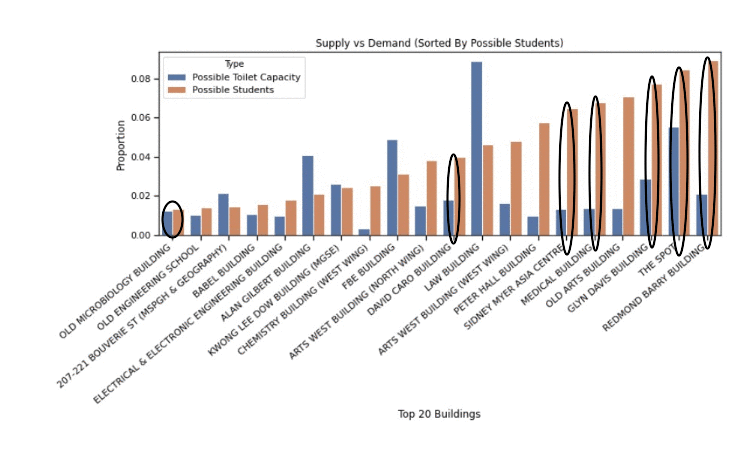
\includegraphics[width=10cm,keepaspectratio=true]{resources/images/floor_to/select_buildings.png}
\caption{Supply vs Demand Problem in Parkville Campus}
\label{fig:floor_to}
\end{figure}

% \paragraph{Redmond Barry Building (Parkville Campus)}
% This section discusses about the findings with respect to Redmond Barry Building for supply and demand analysis, and the current location is set as \texttt{Level 2}.
% \begin{itemize}
%     \item \textbf{Best nearby floors with no preference:}
%     As given in the Appendix Table \ref{appendix:redmond_floor_to}, a student needs to walk at least \texttt{2 levels} in the building to get rewarding floors with sufficient supply of toilets. The results also suggests a relaxing parameter ($\delta$) of \texttt{1} and the students will not miss out floors with high rewards. Using these conditions, the result suggests that \texttt{Level 4} as the most rewarding floor with the cost of \texttt{2 floors} followed by \texttt{Level 6} with \texttt{4 floors} and \texttt{Level 5} with \texttt{3 floors} as shown in the Figure \ref{fig:remond_no}.
%     \begin{figure}[H]
%     \centering
%     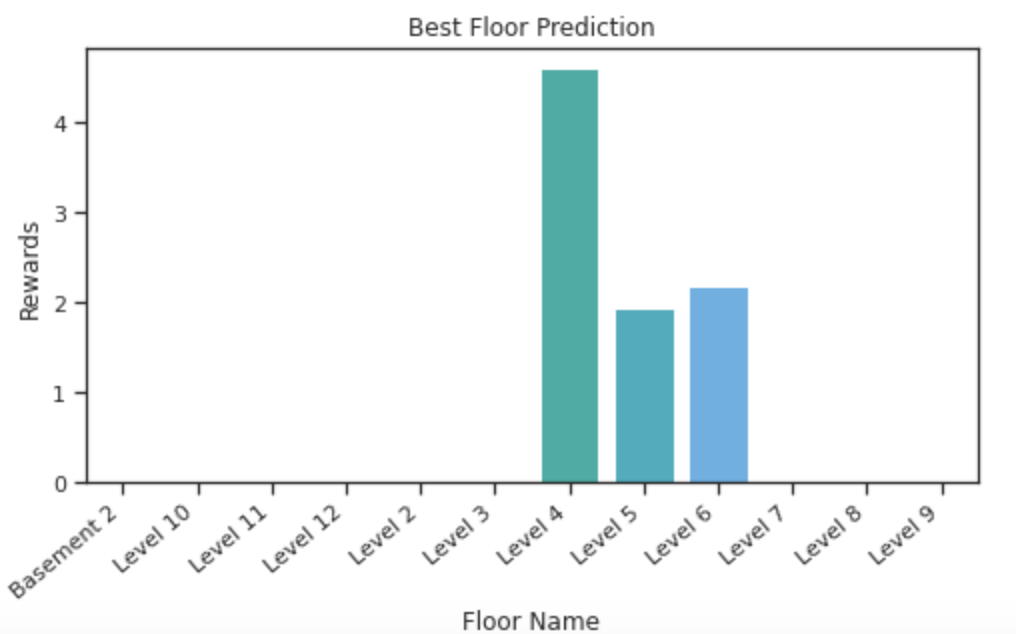
\includegraphics[width=10cm,keepaspectratio=true]{resources/images/floor_to/redmond_no.png}
%     \caption{Best rewarding floors of Redmond Barry Building with no preference}
%     \label{fig:remond_no}
%     \end{figure}
    
%     \item \textbf{Best nearby floors under COVID-19 Strict Lockdown:}
%     Based on the Appendix Table \ref{appendix:redmond_floor_to}, we find out that a student needs to walk at least \texttt{1 level} in the building to get rewarding floors with sufficient supply of toilets during strict lockdown. It is suggested that a relaxing parameter ($\delta$) of \texttt{3} can help students find highly rewarding floors. The result indicates that \texttt{Level 4} as the most rewarding floor with the cost of \texttt{2 floors} followed by \texttt{Level 1} with \texttt{3 floors} and \texttt{Basement 2} with \texttt{4 floors} as shown in the Figure \ref{fig:remond_covidhigh}.
    
%     \begin{figure}[H]
%     \centering
%     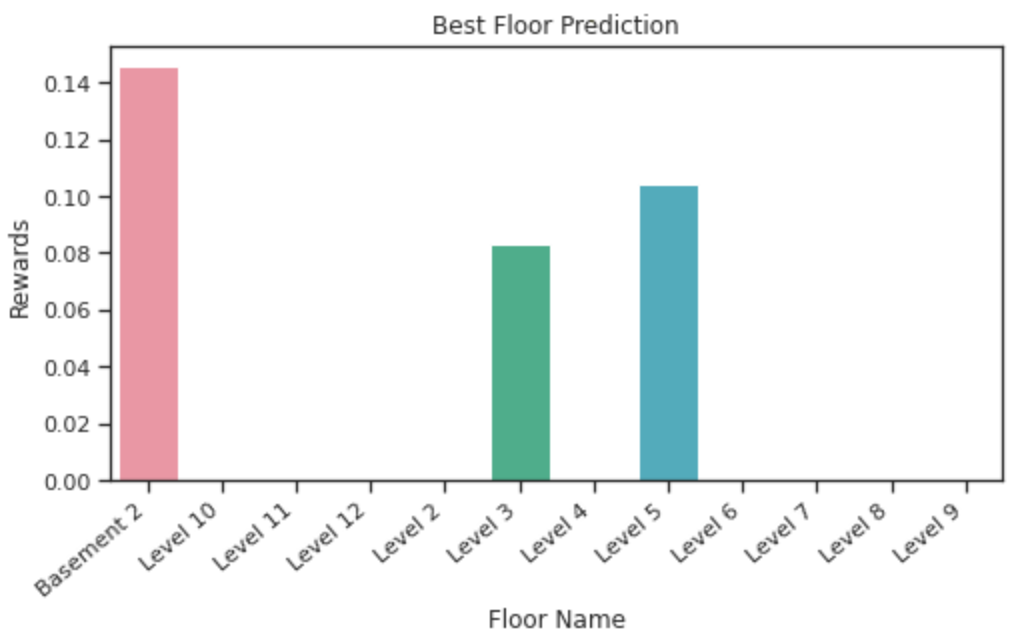
\includegraphics[width=10cm,keepaspectratio=true]{resources/images/floor_to/redmond_covidhigh.png}
%     \caption{Best rewarding floors of Redmond Barry Building under COVID-19 Strict Lockdown}
%     \label{fig:remond_covidhigh}
%     \end{figure}
    
%     \item \textbf{Best nearby floors with toilets in excellent condition:}
%     We find out that a student needs to walk at least \texttt{1 level} in the building to get rewarding floors with sufficient supply of excellent condition toilets from the Appendix Table \ref{appendix:redmond_floor_to}. It is also suggested that a relaxing parameter ($\delta$) of \texttt{1} can help students find highly rewarding floors. The result indicates that \texttt{Level 4} as the most rewarding floor with the cost of \texttt{2 floors} followed by \texttt{Level 5} with \texttt{3 floors} and \texttt{Level 3} with \texttt{4 floors} as shown in the Figure \ref{fig:remond_ex}.
    
%     \begin{figure}[H]
%     \centering
%     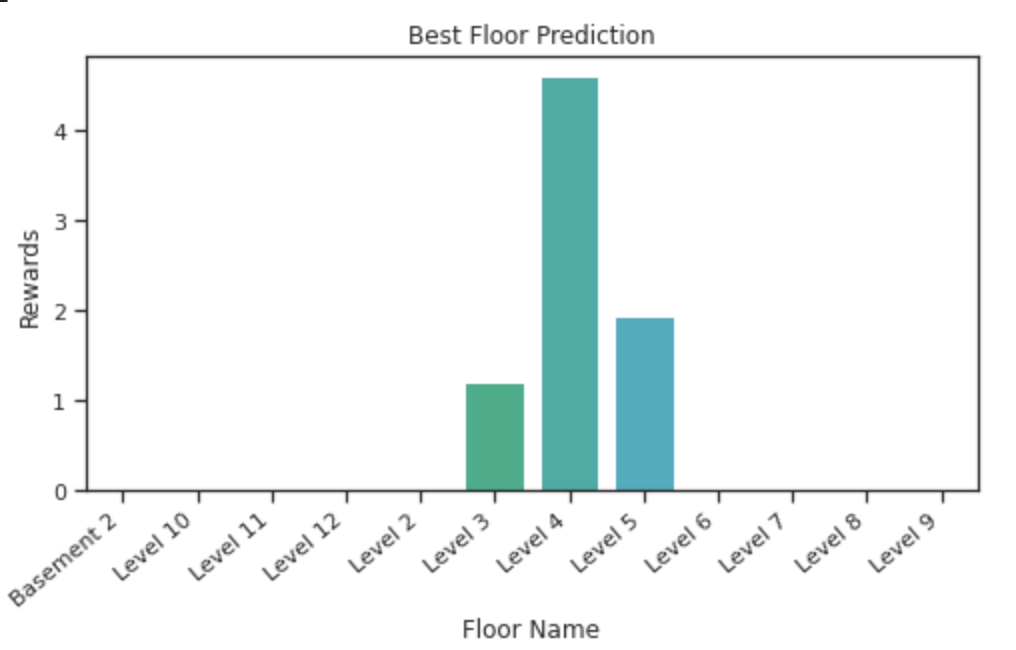
\includegraphics[width=10cm,keepaspectratio=true]{resources/images/floor_to/redmond_excellent.png}
%     \caption{Best rewarding floors of Redmond Barry Building with excellent condition toilets}
%     \label{fig:remond_ex}
%     \end{figure}
    
%     \item \textbf{Best nearby floors with other factors:}
%     In the Appendix Table \ref{appendix:redmond_floor_to}, we have also shown other factors such as finding toilets with easy availability and high capacity. Using those constraints, we suggest that \texttt{Level 4} is the most rewarding floor with finding toilets with easy availability, or high capacity. These are summarized in the below figures.
%     \begin{figure}[H]
% \centering
% \begin{subfigure}[b]{0.30\textwidth}
%   \centering
%   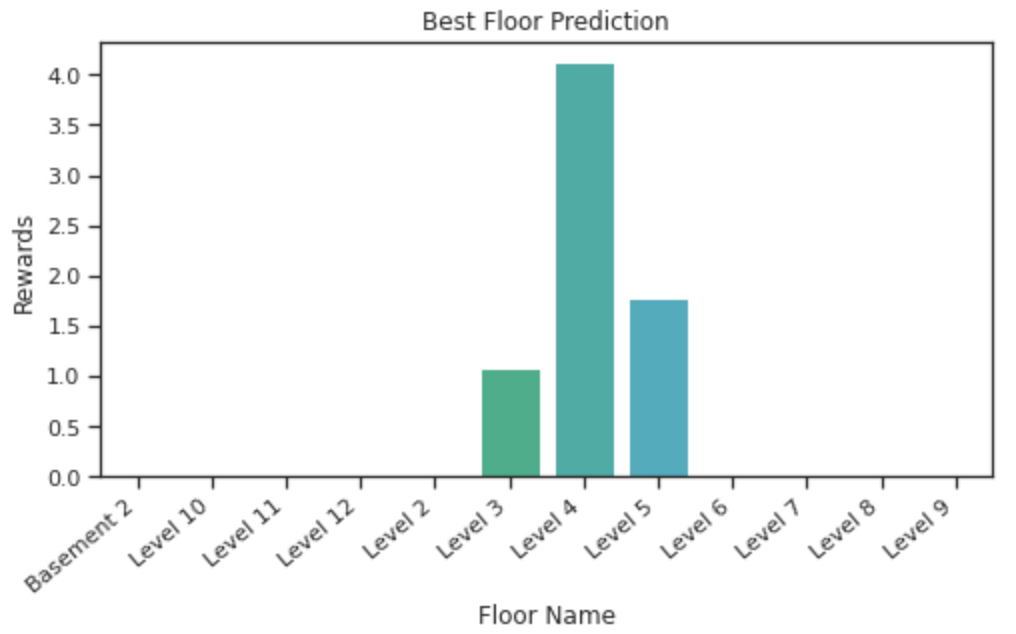
\includegraphics[width=4.5cm,keepaspectratio=true]{resources/images/floor_to/remond_easyava.png}
% \end{subfigure}
% \begin{subfigure}[b]{0.30\textwidth}
%   \centering
%   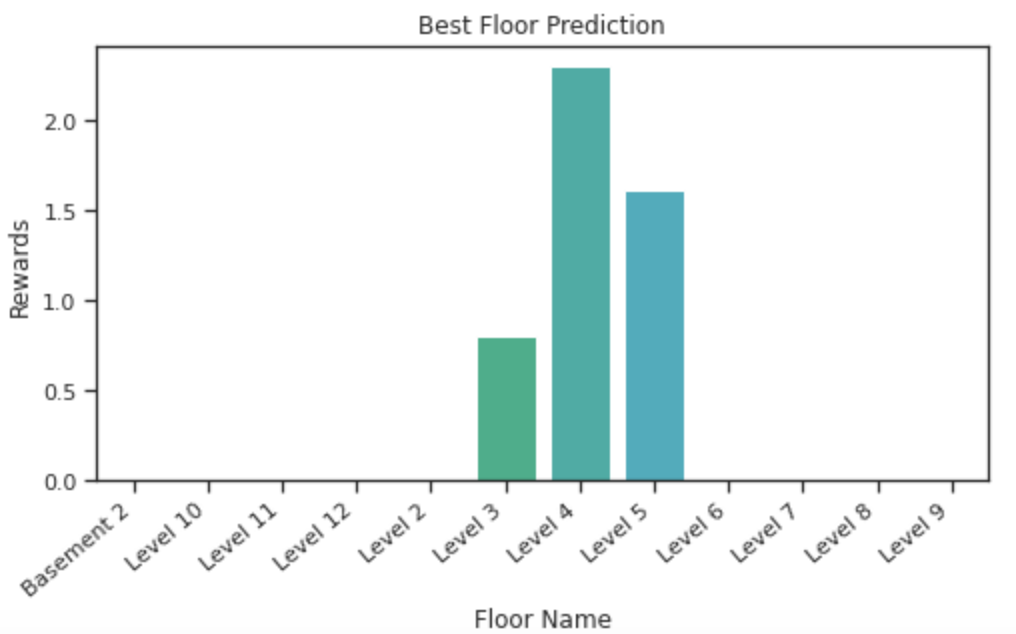
\includegraphics[width=4.5cm,keepaspectratio=true]{resources/images/floor_to/remond_highcap.png}
% \end{subfigure}

% \caption{Best rewarding floors of nearby floors of Redmond Barry Building based on availability (left) and capacity (right)}
% \label{fig:redmond-other-factors}
% \end{figure}
%     \end{itemize}


% \paragraph{The Spot (Parkville Campus)}
% This section discusses about the findings with respect to The Spot for supply and demand analysis, and the current location is set as \texttt{Level 3}.
% \begin{itemize}
%     \item \textbf{Best nearby floors with no preference:}
%     In the Appendix Table \ref{appendix:spot_floor_to}, we conclude that a student needs to walk at least \texttt{1 level} in the building to get rewarding floors with sufficient supply of toilets. It is suggested that a relaxing parameter ($\delta$) of \texttt{2} can help students find highly rewarding floors. The result indicates that \texttt{Level 1} as the most rewarding floor with the cost of \texttt{2 floors} followed by \texttt{Level 6} with \texttt{3 floors} and \texttt{Level 4} with \texttt{1 floor} as shown in the Figure \ref{fig:spot_no}.
    
%     \begin{figure}[H]
%     \centering
%     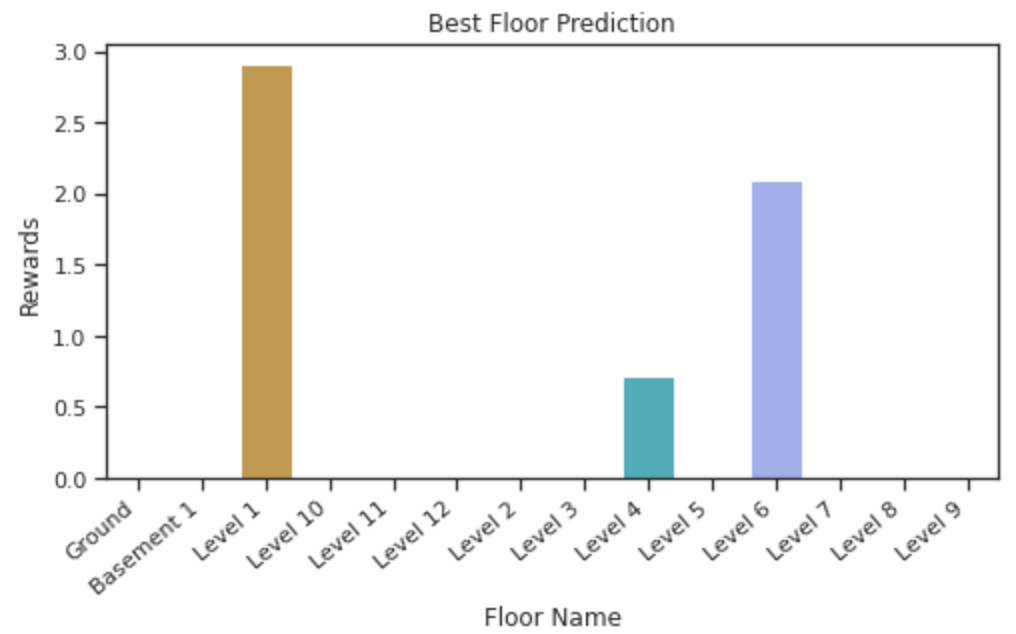
\includegraphics[width=10cm,keepaspectratio=true]{resources/images/floor_to/spot_no.png}
%     \caption{Best rewarding floors of The Spot with no preference}
%     \label{fig:spot_no}
%     \end{figure}
    
%     \item \textbf{Best nearby floors with high capacity:}
%     To find a floor with high capacity in toilets, from the Appendix Table \ref{appendix:spot_floor_to}, we find out that a student needs to walk at least \texttt{1 level} in the building to get rewarding floors. It is also revealed that a relaxing parameter ($\delta$) of \texttt{3} can help students find highly rewarding floors. The result indicates that \texttt{Level 1} as the most rewarding floor with the cost of \texttt{2 floors} followed by \texttt{Level 4} with \texttt{1 floor} and \texttt{Level 2} with \texttt{1 floor} as shown in the Figure \ref{fig:spot_highcap}.
%     \begin{figure}[H]
%     \centering
%     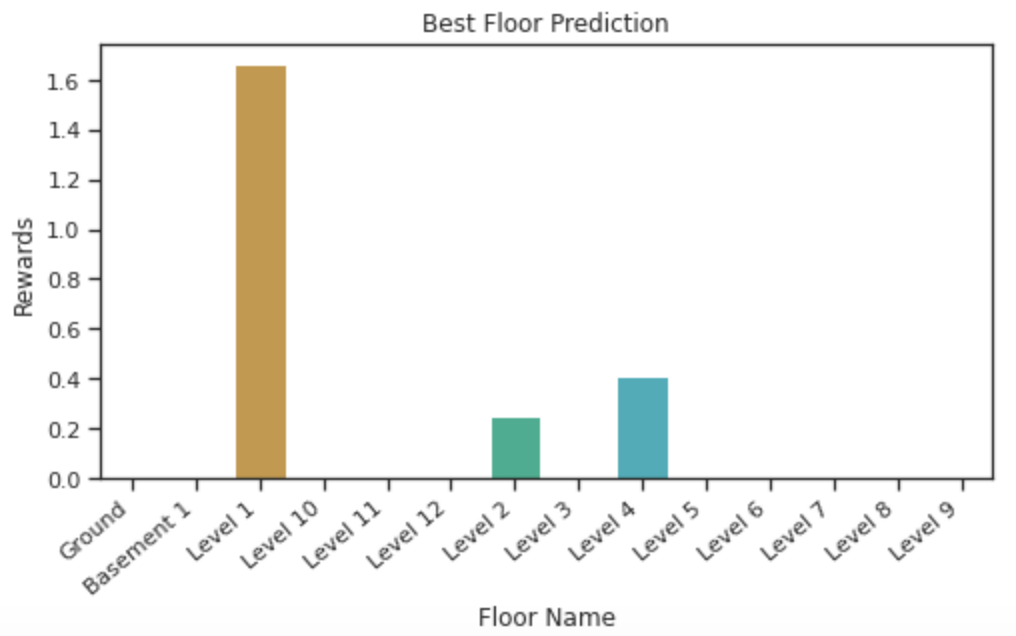
\includegraphics[width=10cm,keepaspectratio=true]{resources/images/floor_to/spot_highcap.png}
%     \caption{Best rewarding floors of The Spot with high capacity}
%     \label{fig:spot_highcap}
%     \end{figure}
    
%     \item \textbf{Best nearby floors with easy availability:}
%      Based on the Appendix Table \ref{appendix:spot_floor_to}, a student needs to walk at least \texttt{1 level} in the building to get rewarding floors with easy availability. It is also suggested that a relaxing parameter ($\delta$) of \texttt{1} can help students find highly rewarding floors. The result indicates that \texttt{Level 1} as the most rewarding floor with the cost of \texttt{2 floors} followed by \texttt{Level 6} with \texttt{3 floors} and \texttt{Level 4} with \texttt{1 floor} as shown in the Figure \ref{fig:spot_easyava}.
    
%     \begin{figure}[H]
%     \centering
%     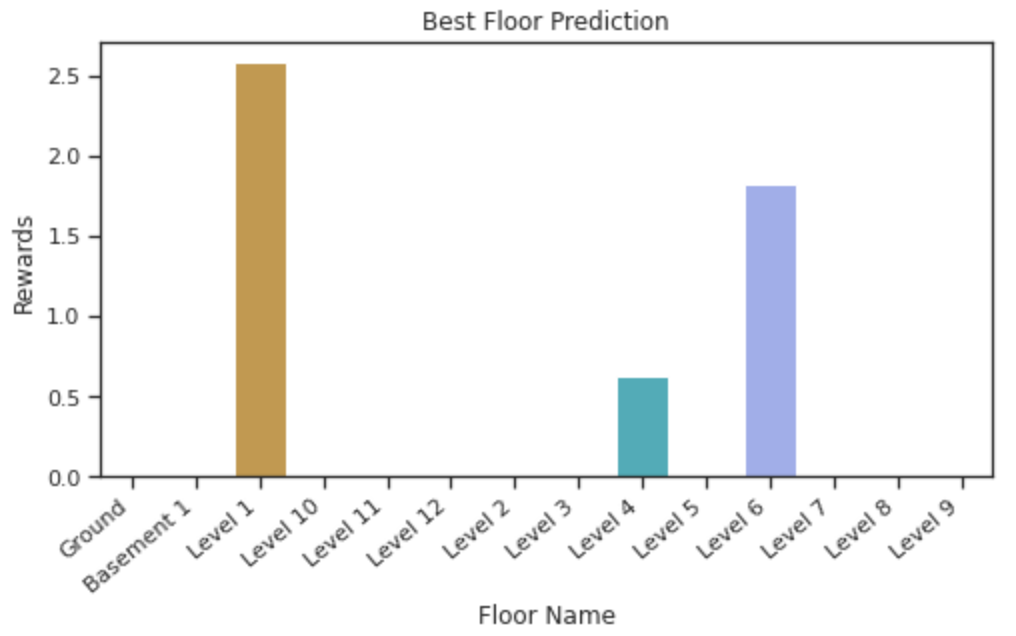
\includegraphics[width=10cm,keepaspectratio=true]{resources/images/floor_to/spot_easyava.png}
%     \caption{Best rewarding floors of The Spot with easy availability}
%     \label{fig:spot_easyava}
%     \end{figure}
    
    
%     \item\textbf{Best nearby floors with other factors:}
%     From the Appendix Table \ref{appendix:spot_floor_to}, we have also shown other factors, including COVID-19 Low Lockdown situation and toilets with excellent condition. Using those constraints, we suggest that \texttt{Level 1} is the most rewarding floor with finding toilets under COVID-19 Low Lockdown, and with excellent condition. These are summarized in the below figures.
   
% \begin{figure}[H]
% \centering
% \begin{subfigure}[b]{0.30\textwidth}
%   \centering
%   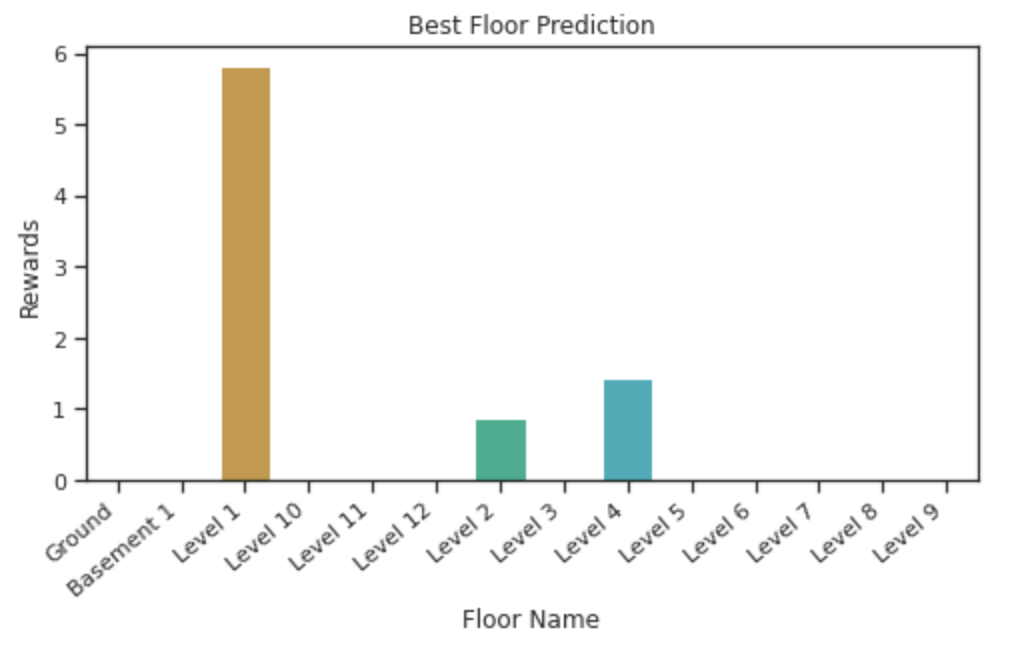
\includegraphics[width=4.5cm,keepaspectratio=true]{resources/images/floor_to/spot_covidlow.png}
% \end{subfigure}
% \begin{subfigure}[b]{0.30\textwidth}
%   \centering
%   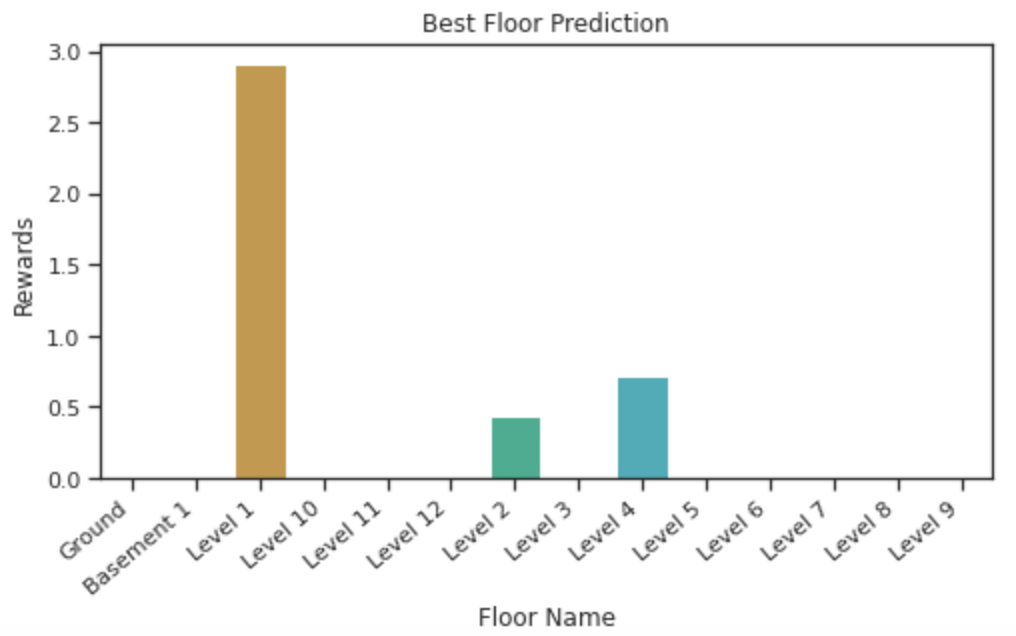
\includegraphics[width=4.5cm,keepaspectratio=true]{resources/images/floor_to/spot_excellent.png}
% \end{subfigure}
% \caption{Best rewarding floors of nearby floors of The Spot under COVID-19 Low Lockdown (left) and excellent condition (right)}
% \label{fig:spot-other-factors}
% \end{figure}
% \end{itemize}


% \paragraph{Glyn Davis Building (Parkville Campus)}
% This section discusses about the findings with respect to Glyn Davis Building for supply and demand analysis, and the current location is set as \texttt{Ground}.
% \begin{itemize}
%     \item \textbf{Best nearby floors with no preference:}
%     As given in the Appendix Table \ref{appendix:glyn_floor_to}, a student needs to walk at least \texttt{1 level} in the building to get rewarding floors with adequate supply of toilets. The results also suggests a relaxing parameter ($\delta$) of \texttt{2} and the students will not miss out floors with high rewards. Using these conditions, the result suggests that \texttt{Level 3} as the most rewarding floor with the cost of \texttt{3 floors} followed by \texttt{Level 2} with \texttt{2 floors} and \texttt{Level 1} with \texttt{1 floor} as shown in the Figure \ref{fig:gyln_no}.
    
%     \begin{figure}[H]
%     \centering
%     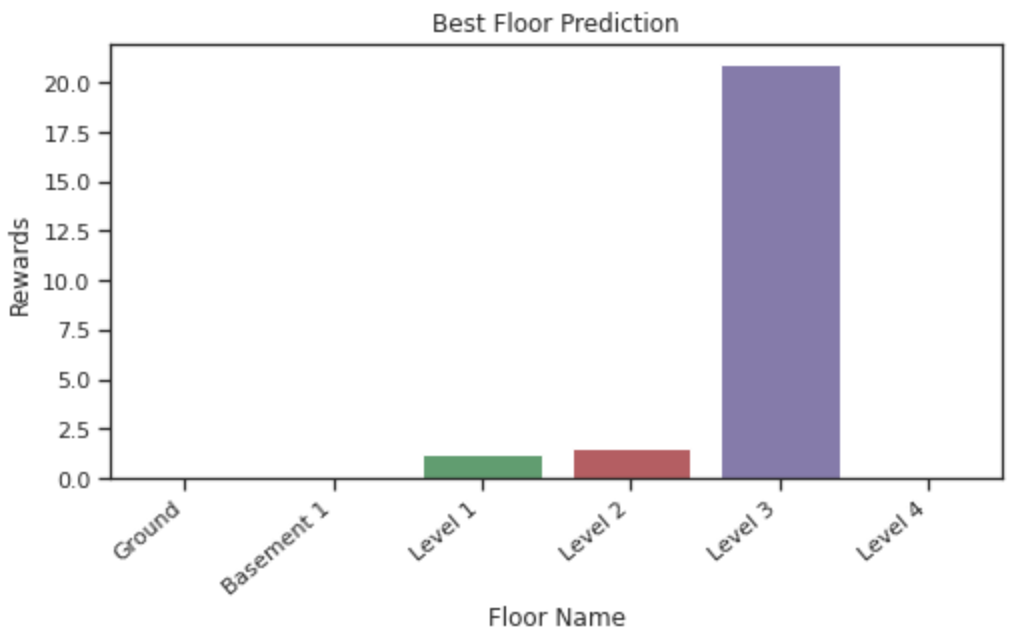
\includegraphics[width=10cm,keepaspectratio=true]{resources/images/floor_to/gyln_no.png}
%     \caption{Best rewarding floors of Glyn Davis Building no preference}
%     \label{fig:gyln_no}
%     \end{figure}
    
%     \item \textbf{Best nearby floors under COVID-19 Strict Lockdown:}
%     Based on the Appendix Table \ref{appendix:glyn_floor_to}, a student needs to walk at least \texttt{1 level} in the building to get rewarding floors under strict lockdown. It is also suggested that a relaxing parameter ($\delta$) of \texttt{1} can help students find highly rewarding floors. The result indicates that \texttt{Basement 1} as the most rewarding floor with the cost of \texttt{1 floor} followed by \texttt{Level 2} with \texttt{2 floors} and \texttt{Level 1} with \texttt{1 floor} as shown in the Figure \ref{fig:gyln_covidhigh}.
%     \begin{figure}[H]
%     \centering
%     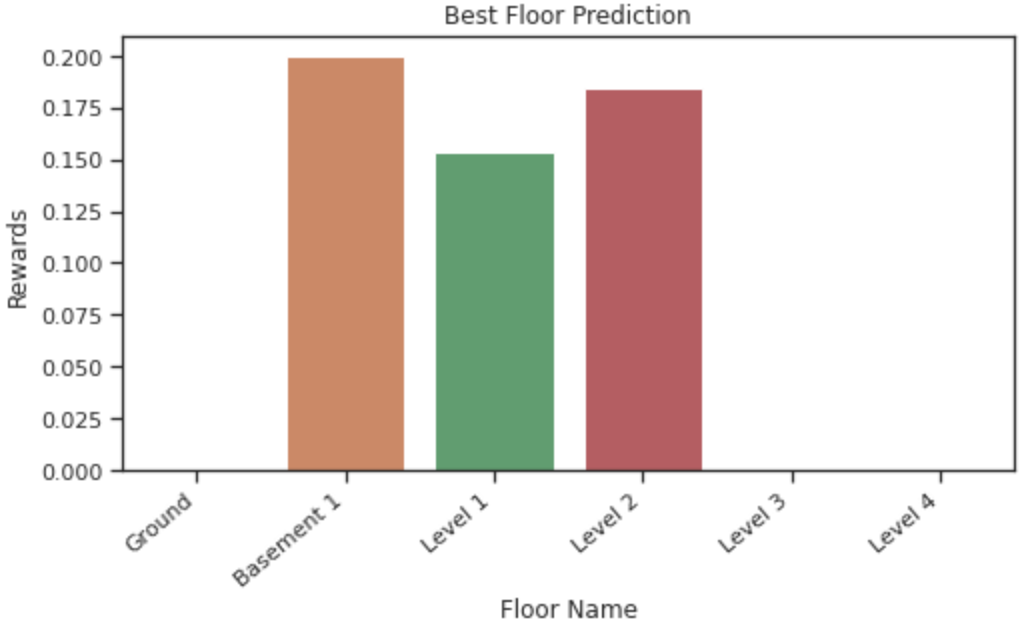
\includegraphics[width=10cm,keepaspectratio=true]{resources/images/floor_to/gyln_covidhigh.png}
%     \caption{Best rewarding floors of Glyn Davis Building under COVID-19 Strict Lockdown}
%     \label{fig:gyln_covidhigh}
%     \end{figure}
    
%     \item \textbf{Best nearby floors with easy availability:}
%     From the Appendix Table \ref{appendix:glyn_floor_to}, we find that a student needs to walk at least \texttt{2 levels} in the building to get rewarding floors with easy availability. It is also suggested that a relaxing parameter ($\delta$) of \texttt{2} can help students find highly rewarding floors. The result indicates that \texttt{Level 3} as the most rewarding floor with the cost of \texttt{3 floors} followed by \texttt{Level 4} with \texttt{4 floors} and \texttt{Level 2} with \texttt{2 floor} as shown in the Figure \ref{fig:gyln_easyava}.
    
%     \begin{figure}[H]
%     \centering
%     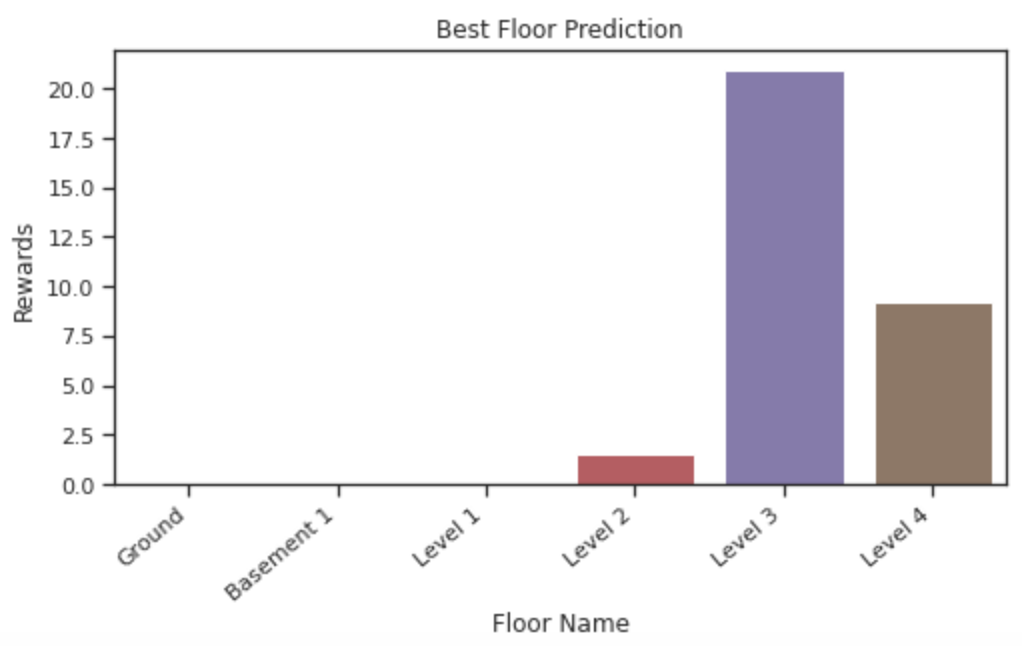
\includegraphics[width=10cm,keepaspectratio=true]{resources/images/floor_to/gyln_easyava.png}
%     \caption{Best rewarding floors of Glyn Davis Building with easy availability}
%     \label{fig:gyln_easyava}
%     \end{figure}
    
%     \item \textbf{Best nearby floors with other factors:}
%     We have also evaluated other factors such as finding toilets with high capacity and excellent condition in the Appendix Table \ref{appendix:glyn_floor_to}. Using those constraints, we suggest that \texttt{Level 3} is the most rewarding floor with finding toilets with high capacity, or excellent condition. These are summarized in the below figures.
    
% \begin{figure}[H]
% \centering
% \begin{subfigure}[b]{0.30\textwidth}
%   \centering
%   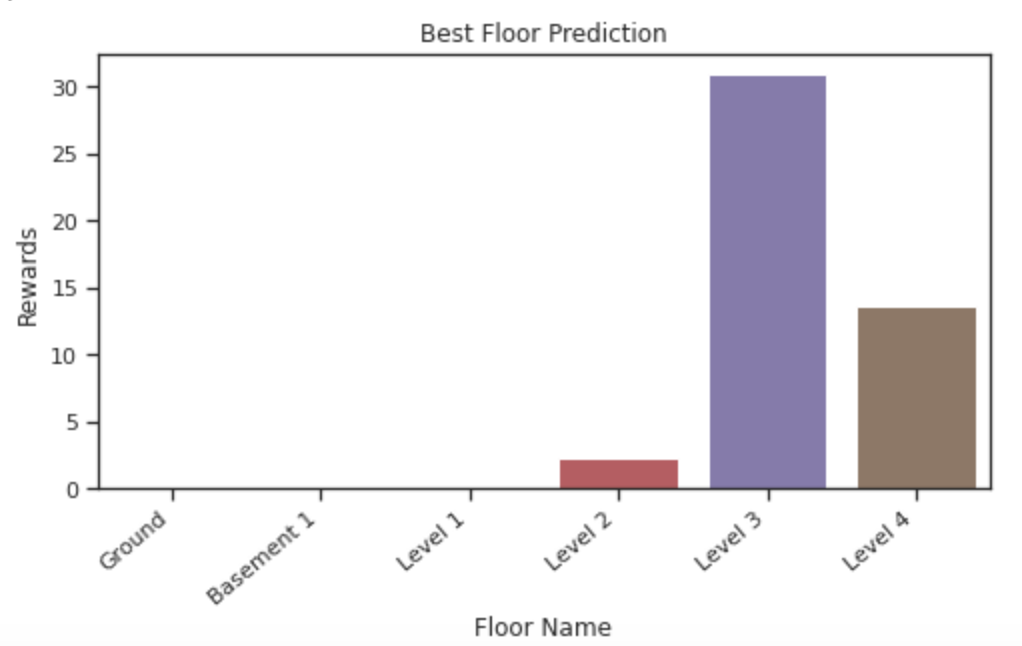
\includegraphics[width=4.5cm,keepaspectratio=true]{resources/images/floor_to/gyln_highcap.png}
% \end{subfigure}
% \begin{subfigure}[b]{0.30\textwidth}
%   \centering
%   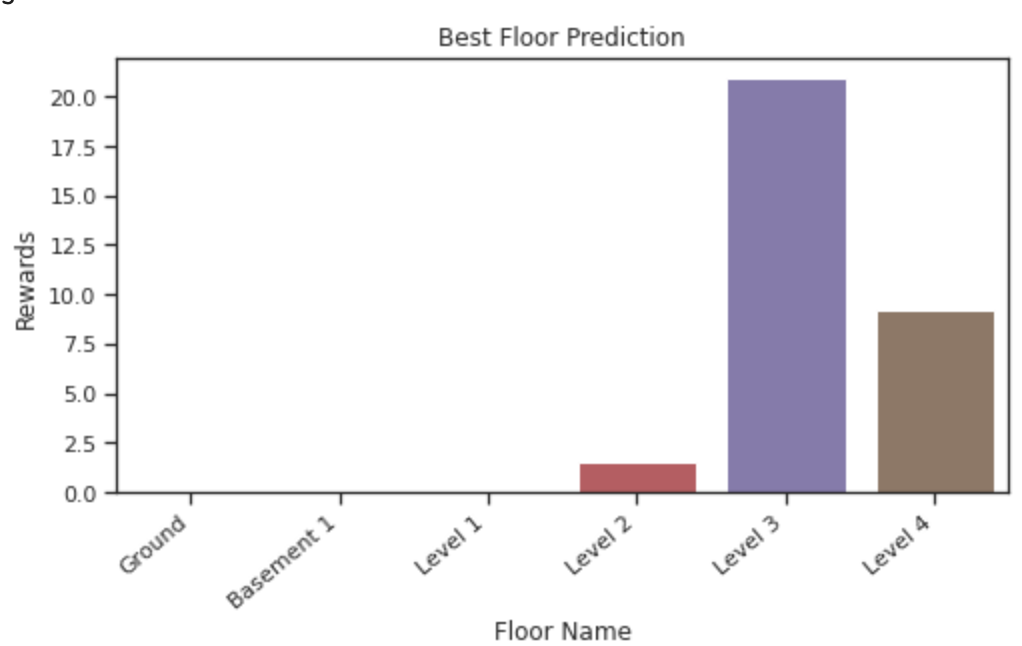
\includegraphics[width=4.5cm,keepaspectratio=true]{resources/images/floor_to/gyln_excellent.png}
% \end{subfigure}
% \caption{Best rewarding floors of nearby floors of Glyn Davis Building with high capacity (left) and excellent condition (right)}
% \label{fig:spot-other-factors}
% \end{figure}
% \end{itemize}
    

\paragraph{Medical Building (Parkville Campus)}
This section discusses the findings with respect to Medical Building for supply and demand analysis, and the current location is set as \texttt{Level 5}.
\begin{itemize}
    \item \textbf{Best nearby floors with no preference:}
    The Appendix Table \ref{appendix:medical_floor_to} shows that a student needs to walk at least \texttt{1 level} in the building to get rewarding floors. It is also suggested that a relaxing parameter ($\delta$) of \texttt{3} can help students find highly rewarding floors. The most rewarding floor is \texttt{Level 7} and followed by \texttt{Level 9, Level 2} in order with costs \texttt{2, 4, 3 floors}.
    \begin{figure}[H]
    \centering
    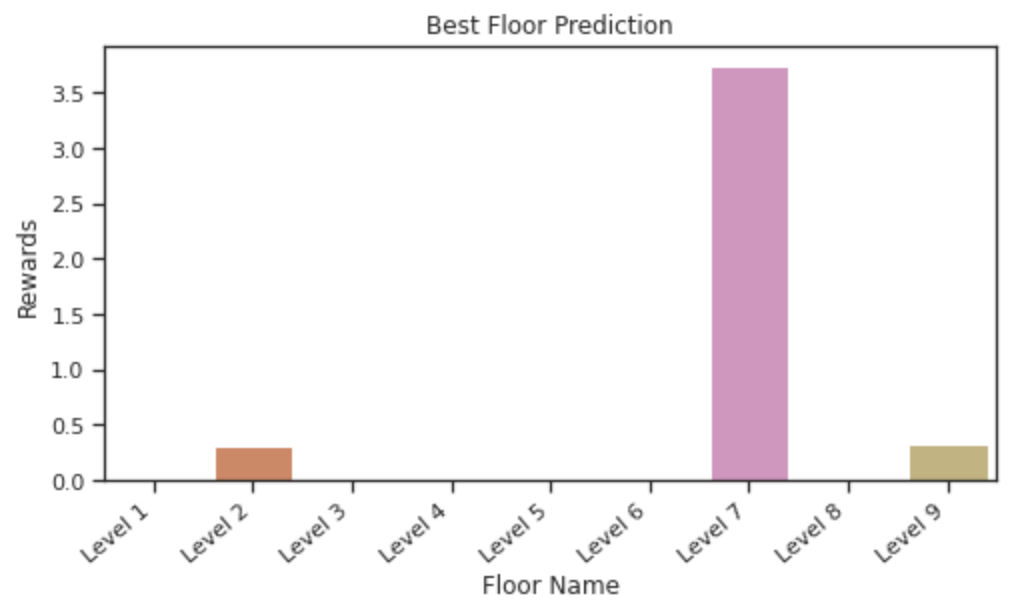
\includegraphics[width=10cm,keepaspectratio=true]{resources/images/floor_to/medical_no.png}
    \caption{Best rewarding floors of Medical Building with no preference}
    \label{fig:medical_no}
    \end{figure}
    
    \item \textbf{Best nearby floors with high capacity:} From the Appendix Table \ref{appendix:medical_floor_to}, we find out that a student needs to walk at least \texttt{1 level} in the building to get rewarding floors with high capacity. It is also suggested that a relaxing parameter ($\delta$) of \texttt{3} can help students find better rewarding floors. The result indicates that \texttt{Level 1} as the most rewarding floor with the cost of \texttt{4 floors} followed by \texttt{Level 7} with \texttt{2 floors} and \texttt{Level 9} with \texttt{4 floors} as shown in the Figure \ref{fig:medical_highcap}.
    
    \begin{figure}[H]
    \centering
    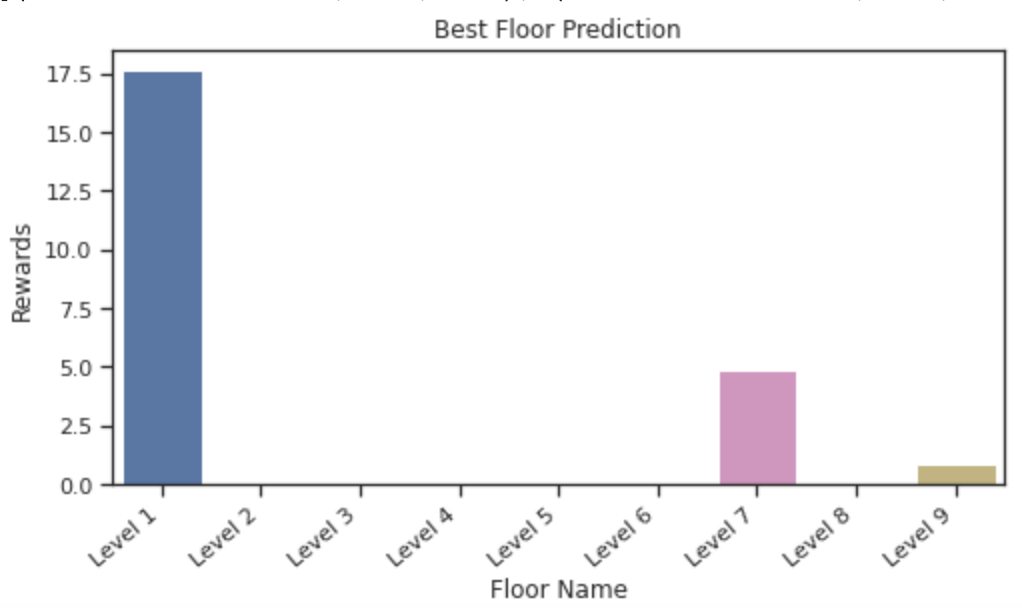
\includegraphics[width=10cm,keepaspectratio=true]{resources/images/floor_to/medical_highcap.png}
    \caption{Best rewarding floors of Medical Building with high capacity}
    \label{fig:medical_highcap}
    \end{figure}
    
%    \item \textbf{Best nearby floors with excellent toilet condition:}
%    To access toilets with excellent condition, the Appendix Table \ref{appendix:medical_floor_to} shows that a student needs to walk at least \texttt{2 level} in the building to get rewarding floors. It is also suggested that a relaxing parameter ($\delta$) of \texttt{2} can help students find highly rewarding floors. The result indicates that \texttt{Level 1} as the most rewarding floor with the cost of \texttt{4 floors} followed by \texttt{Level 7} with \texttt{2 floors} and \texttt{Level 9} with \texttt{4 floors} as shown in the Figure \ref{fig:medical_excellent}.
    
%    \begin{figure}[H]
%    \centering
%    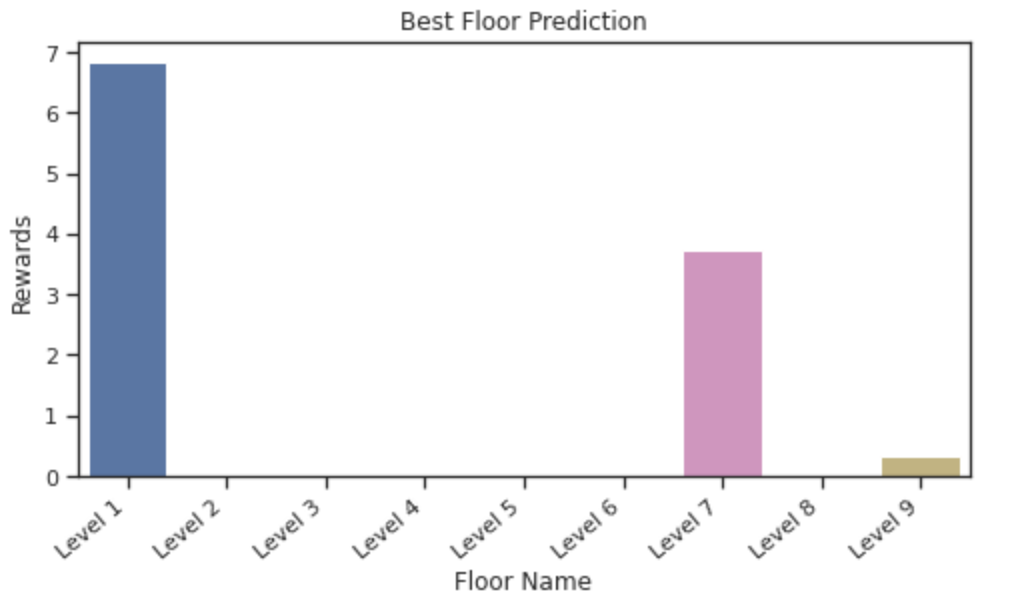
\includegraphics[width=10cm,keepaspectratio=true]{resources/images/floor_to/medical_excellent.png}
%    \caption{Best rewarding floors of Medical Building with excellent toilet condition}
%    \label{fig:medical_excellent}
%    \end{figure}
    
    \item \textbf{Best nearby floors with other factors:}
    
    Other factors are also evaluated in the Appendix Table \ref{appendix:medical_floor_to}, such as finding toilets with easy availability and under COVID-19 Strict Lockdown. Using those constraints, we suggest that \texttt{Level 7} is the most rewarding floor with finding toilets with easy availability, or under COVID-19 Strict Lockdown. These are summarized in the below figures.
    
    
\begin{figure}[H]
\centering
\begin{subfigure}[b]{0.30\textwidth}
  \centering
  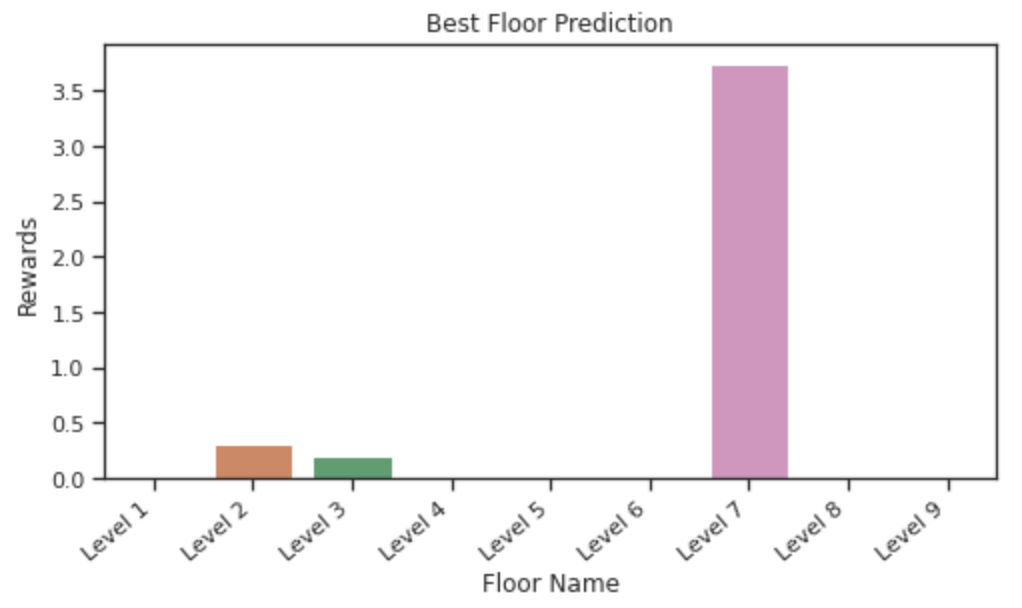
\includegraphics[width=4.5cm,keepaspectratio=true]{resources/images/floor_to/medical_covidmedium.png}
\end{subfigure}
\begin{subfigure}[b]{0.30\textwidth}
  \centering
  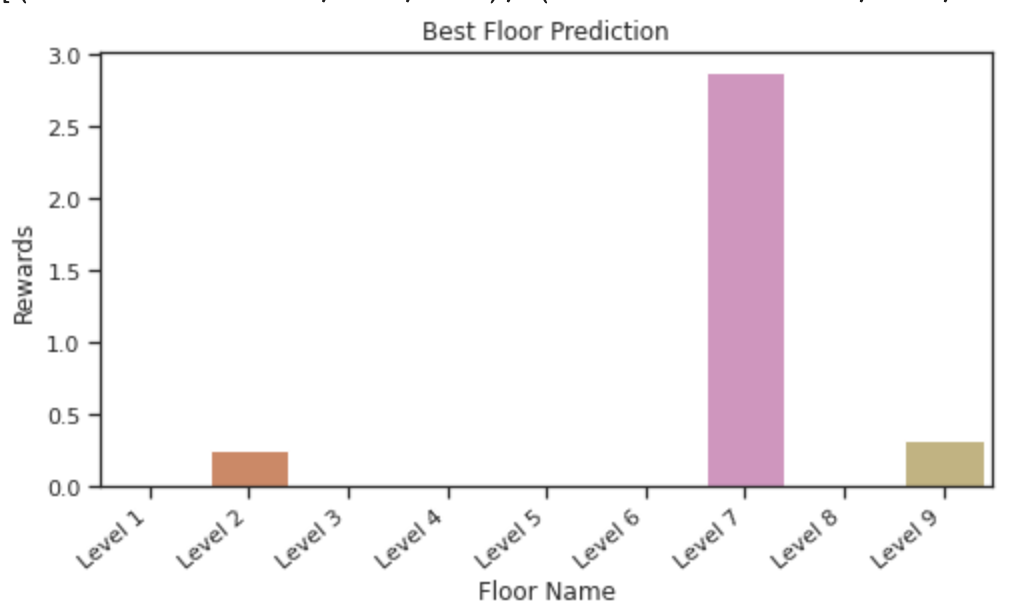
\includegraphics[width=4.5cm,keepaspectratio=true]{resources/images/floor_to/medical_easyava.png}
\end{subfigure}
\caption{Best rewarding floors of nearby floors of Medical Building under COVID-19 Medium Lockdown (left) and easy availability (right)}
\label{fig:medical-other-factors}
\end{figure}
\end{itemize}

\paragraph{David Caro Building (Parkville Campus)}
This section discusses the findings of the David Caro Building for supply and demand analysis, and the current location is set as \texttt{Level 4}.
\begin{itemize}
    \item \textbf{Best nearby floors with no preference:}
    The Appendix Table \ref{appendix:dcaro_floor_to} shows that a student needs to walk at least \texttt{1 level} in the building to get rewarding floors. It is also suggested that a relaxing parameter ($\delta$) of \texttt{1} can help students find highly rewarding floors. The most rewarding floor is \texttt{Level 1} and followed by \texttt{Level 3, Level 2} in order with costs \texttt{3, 1, 2 floors}.
    
    \begin{figure}[H]
    \centering
    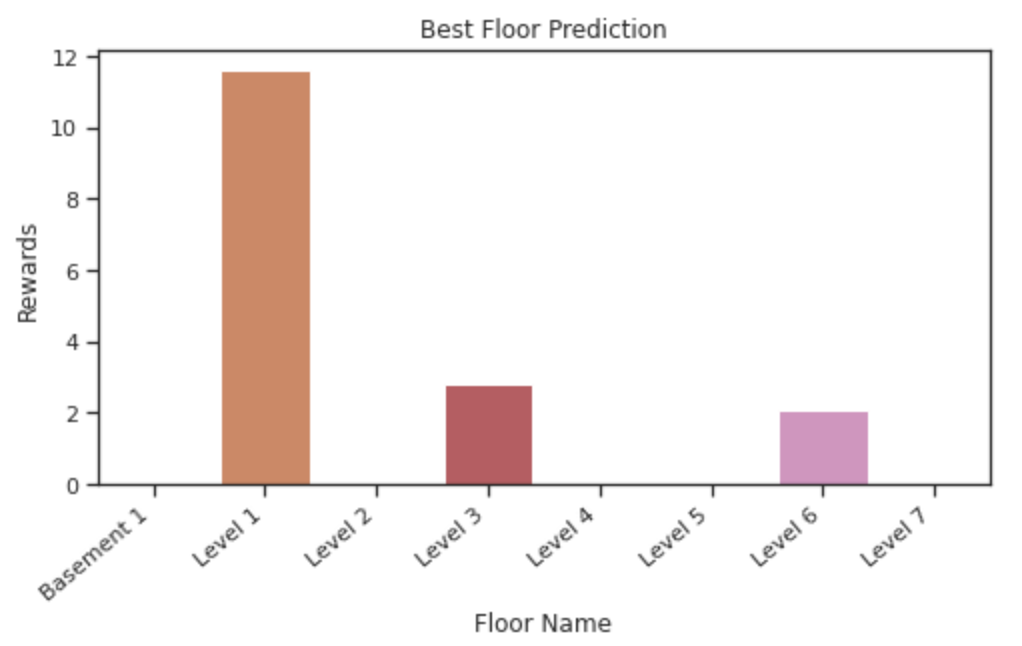
\includegraphics[width=10cm,keepaspectratio=true]{resources/images/floor_to/dcaro_no.png}
    \caption{Best rewarding floors of David Caro Building with no preference}
    \label{fig:dcaro_no}
    \end{figure}
    
    \item \textbf{Best nearby floors under COVID-19 Strict Lockdown:}
    Under COVID-19 Strict Lockdown, we find out that a student needs to walk at least \texttt{1 level} in the building to get rewarding floors with a sufficient supply of toilets based on the Appendix Table \ref{appendix:dcaro_floor_to}. It is suggested that a relaxing parameter ($\delta$) of \texttt{2} can help students find highly rewarding floors. The result indicates that \texttt{Level 2} as the most rewarding floor with the cost of \texttt{3 floors} followed by \texttt{Level 3} with \texttt{1 floor} and \texttt{Level 1} with \texttt{2 floors} as shown in the Figure \ref{fig:dcaro_covidhigh}.
    
    \begin{figure}[H]
    \centering
    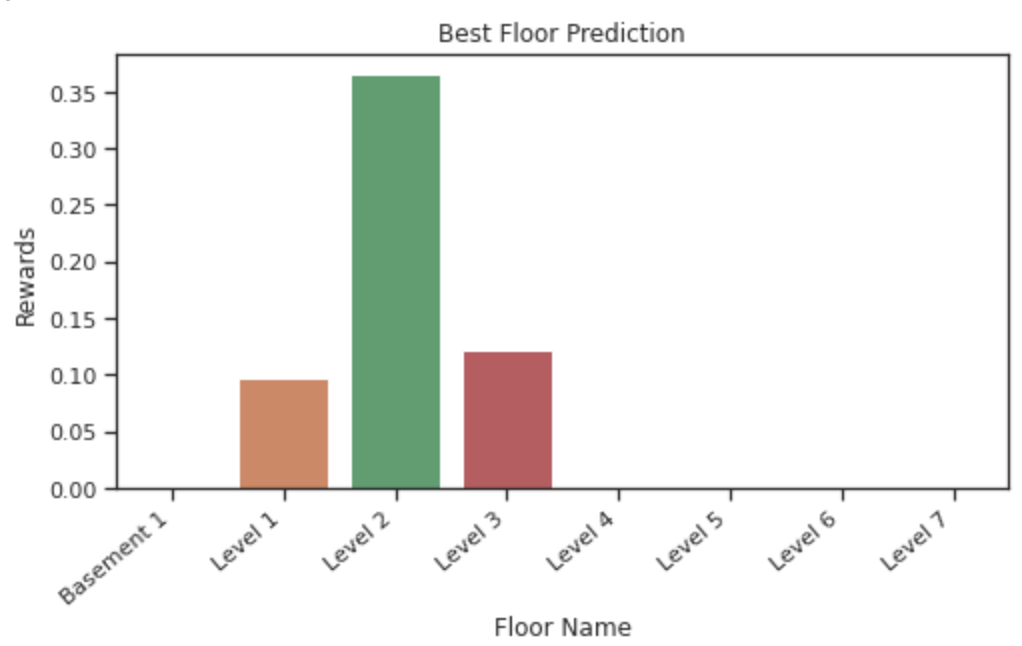
\includegraphics[width=10cm,keepaspectratio=true]{resources/images/floor_to/dcaro_covidhigh.png}
    \caption{Best rewarding floors of David Caro Building under COVID-19 Strict Lockdown}
    \label{fig:dcaro_covidhigh}
    \end{figure}
    
%    \item \textbf{Best nearby floors with high capacity:}
    
%    Based on the Appendix Table \ref{appendix:dcaro_floor_to}, a student needs to walk at least \texttt{1 level} in the building to get rewarding floors with high capacity. It is also suggested that a relaxing parameter ($\delta$) of \texttt{3} can help students find better rewarding floors. The result indicates that \texttt{Level 3} as the most rewarding floor with the cost of \texttt{1 floor} followed by \texttt{Level 6} with \texttt{2 floors} and \texttt{Level 2} with \texttt{2 floors} as shown in the Figure \ref{fig:dcaro_highcap}.
%    \begin{figure}[H]
%    \centering
%    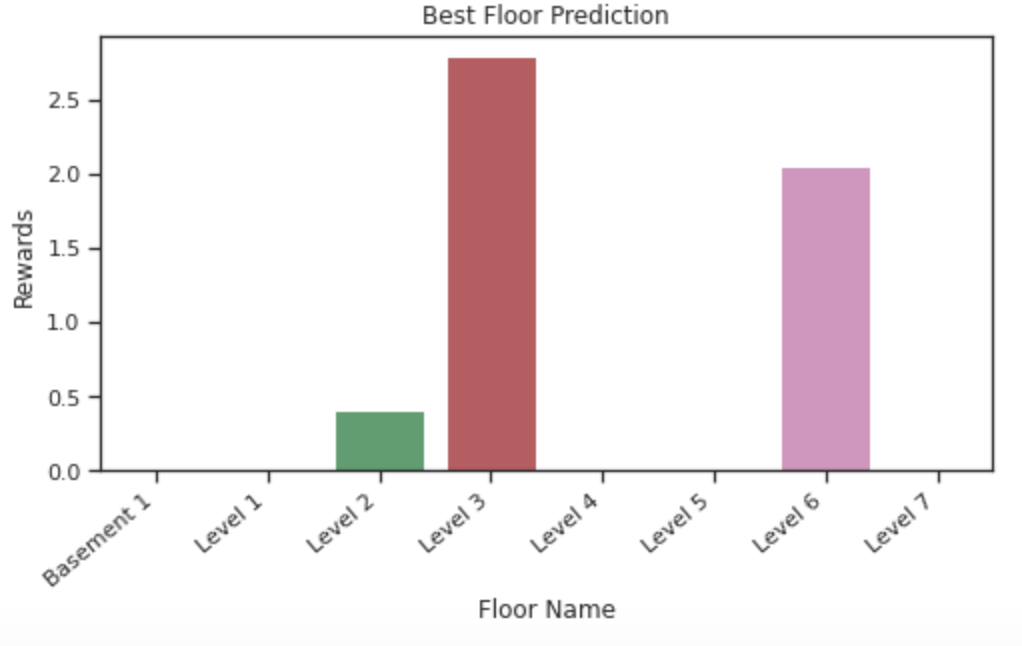
\includegraphics[width=10cm,keepaspectratio=true]{resources/images/floor_to/dcaro_highcap.png}
%    \caption{Best rewarding floors of David Caro Building with high capacity}
%    \label{fig:dcaro_highcap}
%    \end{figure}
    
    \item \textbf{Best nearby floors with other factors:}
    Other factors are also explored, such as finding toilets with easy availability, good condition, and high capacity. Using those constraints, we suggest that \texttt{Level 1} is the most rewarding floor with finding toilets with easy availability, or good condition. These are summarized in the below figures.
    
\begin{figure}[H]
\centering
\begin{subfigure}[b]{0.30\textwidth}
  \centering
  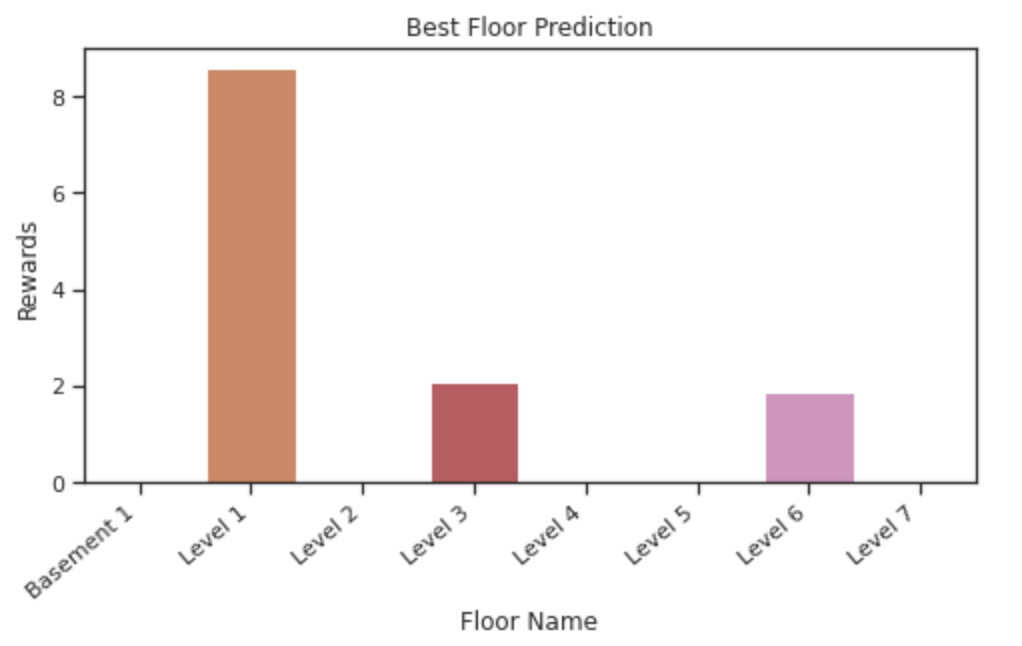
\includegraphics[width=5cm,keepaspectratio=true]{resources/images/floor_to/dcaro_easyava.png}
\end{subfigure}
\begin{subfigure}[b]{0.30\textwidth}
  \centering
  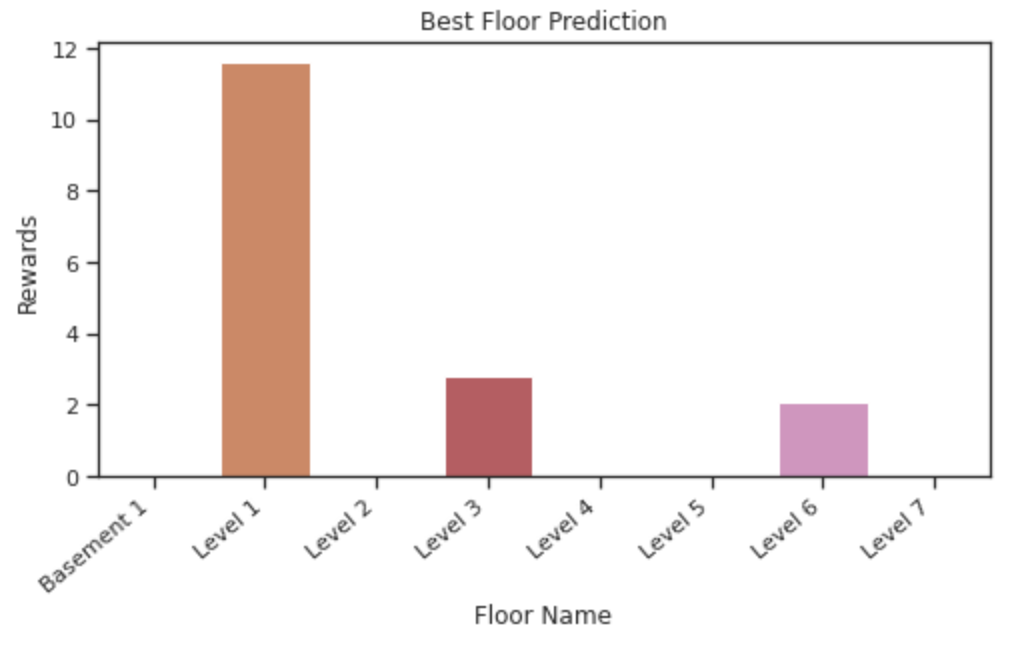
\includegraphics[width=5cm,keepaspectratio=true]{resources/images/floor_to/dcaro_good.png}
\end{subfigure}

\caption{Best rewarding floors of nearby floors of David Caro Building with easy availability (left) and good condition (right)}
\label{fig:dcaro-other-factors}
\end{figure}

\end{itemize}

% \paragraph{Old Microbiology (Parkville Campus)}
% This section discusses about the findings in terms of Old Microbiology for supply and demand analysis, and the current location is set as \texttt{Level 1}.
% \begin{itemize}
%     \item \textbf{Best nearby buildings with no preference:}
%     From the Appendix Table \ref{appendix:oldmicro_floor_to}, we find out that a student needs to walk at least \texttt{1 level} in the building to get rewarding floors with sufficient supply of toilets based on . It is suggested that a relaxing parameter ($\delta$) of \texttt{2} can help students find highly rewarding floors. The result indicates that \texttt{Level 2} as the most rewarding floor with the cost of \texttt{1 floor} followed by \texttt{Ground} with \texttt{1 floor} and \texttt{Level 3} with \texttt{2 floors} as shown in the Figure \ref{fig:dcaro_covidhigh}.
    
%     \begin{figure}[H]
%     \centering
%     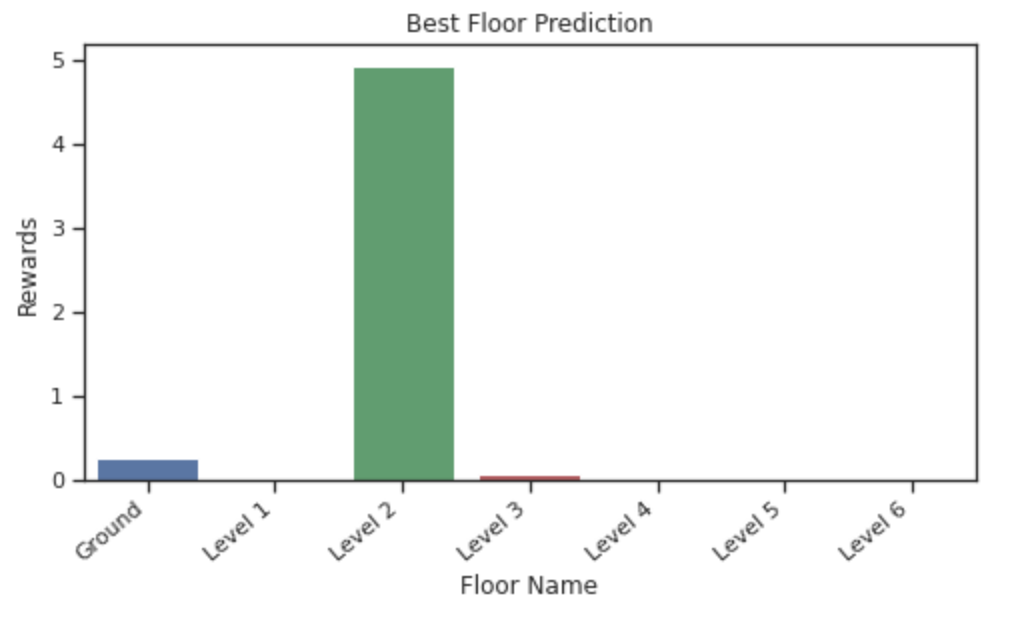
\includegraphics[width=10cm,keepaspectratio=true]{resources/images/floor_to/oldmirco_no.png}
%     \caption{Best rewarding floors of Old Microbiology with no preference}
%     \label{fig:oldmicro_no}
%     \end{figure}
    
%     \item \textbf{Best nearby buildings under COVID-19 Strict Lockdown:}
%     Based on the Appendix Table \ref{appendix:oldmicro_floor_to}, a student needs to walk at least \texttt{1 level} in the building to get rewarding floors during COVID-19 Strict Lockdown. It is also suggested that a relaxing parameter ($\delta$) of \texttt{3} can help students find highly rewarding floors. The most rewarding floor is \texttt{Ground} and followed by \texttt{Level 2, Level 3} in order with costs \texttt{1, 1, 2 floors}.

%     \begin{figure}[H]
%     \centering
%     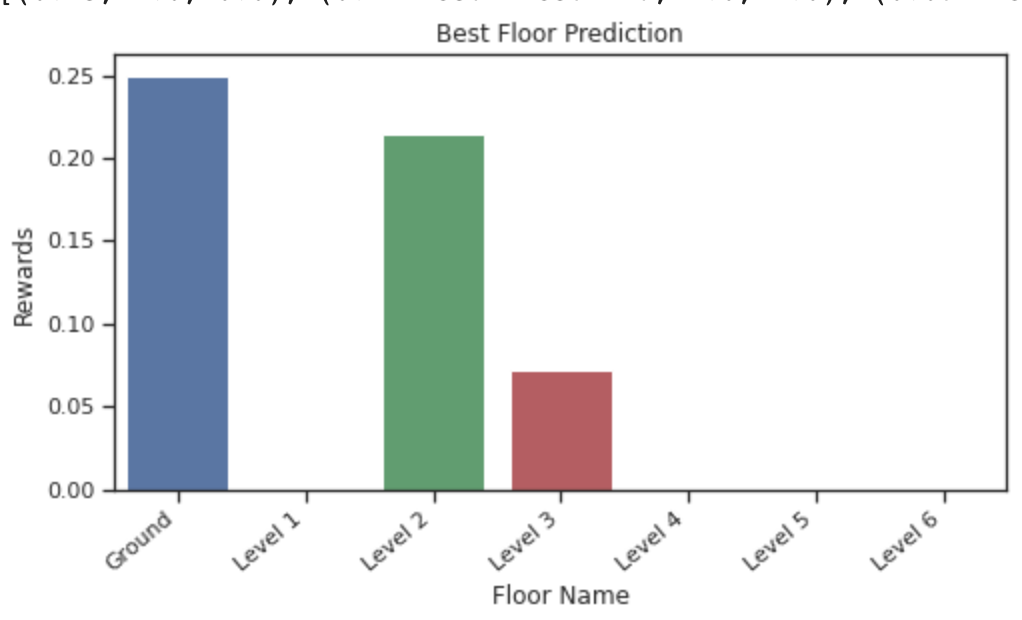
\includegraphics[width=10cm,keepaspectratio=true]{resources/images/floor_to/oldmicro_covidhigh.png}
%     \caption{Best rewarding floors of Old Microbiology under COVID-19 Strict Lockdown}
%     \label{fig:oldmicro_covidhigh}
%     \end{figure}
    
%     \item \textbf{Best nearby buildings with high capacity:}
    
%     From the Appendix Table \ref{appendix:oldmicro_floor_to}, we find out that a student needs to walk at least \texttt{1 level} in the building to get rewarding floors with high capacity. It is also revealed that a relaxing parameter ($\delta$) of \texttt{3} can help students find highly rewarding floors. The result indicates that \texttt{Level 2} as the most rewarding floor with the cost of \texttt{1 floor} followed by \texttt{Ground} with \texttt{1 floor} and \texttt{Level 5} with \texttt{4 floors} as shown in the Figure \ref{fig:oldmicro_highcap}.
%     \begin{figure}[H]
%     \centering
%     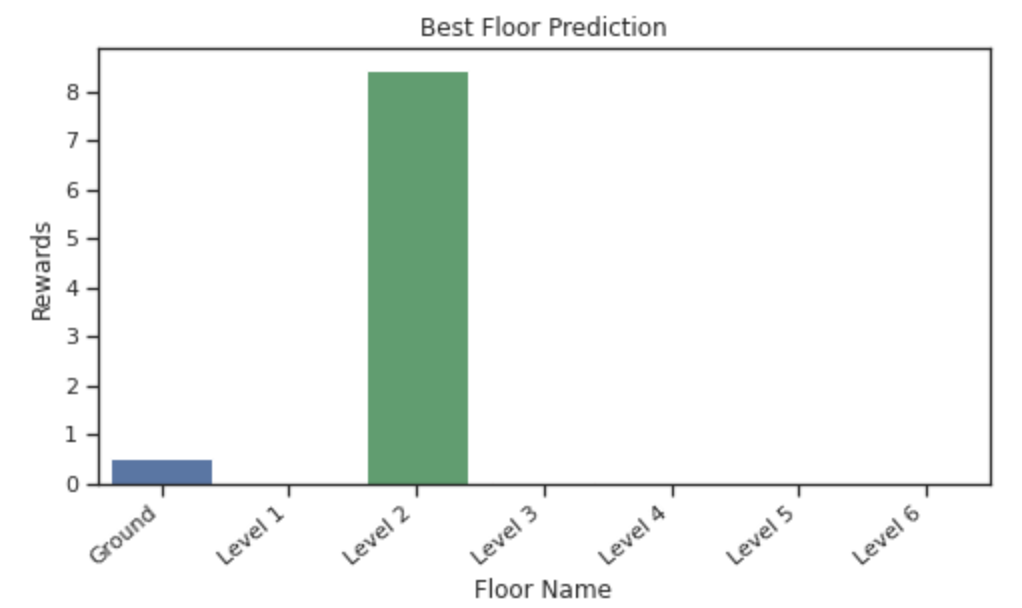
\includegraphics[width=10cm,keepaspectratio=true]{resources/images/floor_to/oldmicro_highcap.png}
%     \caption{Best rewarding floors of Old Microbiology under COVID-19 Strict Lockdown}
%     \label{fig:oldmicro_highcap}
%     \end{figure}
    
%     \item \textbf{Best nearby floors with other factors:}
%     We have also evaluated other factors such as finding toilets with easy availability and good condition in the Appendix Table \ref{appendix:oldmicro_floor_to}. Using those constraints, we suggest that \texttt{Level 2} is the most rewarding floor with finding toilets with easy availability, or good condition. These are summarized in the below figures.
    
% \begin{figure}[H]
% \centering
% \begin{subfigure}[b]{0.30\textwidth}
%   \centering
%   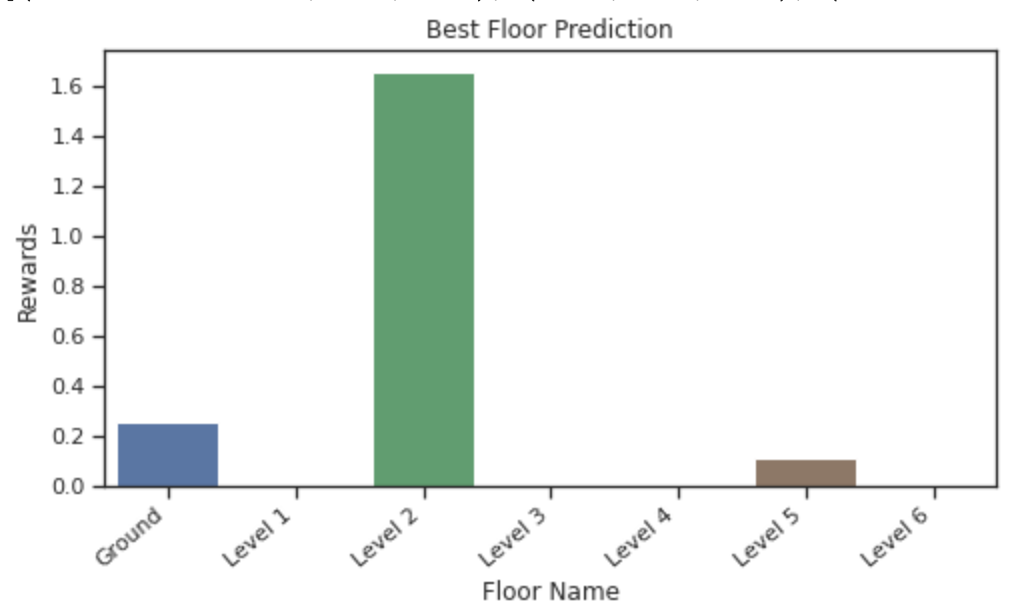
\includegraphics[width=5cm,keepaspectratio=true]{resources/images/floor_to/oldmicro_easyava.png}
% \end{subfigure}
% \begin{subfigure}[b]{0.30\textwidth}
%   \centering
%   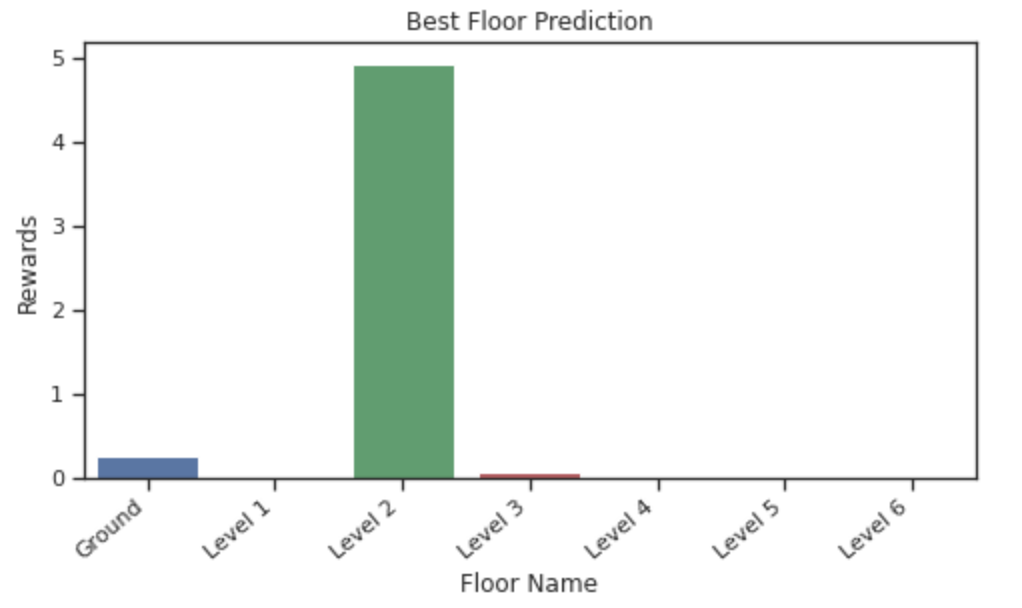
\includegraphics[width=5cm,keepaspectratio=true]{resources/images/floor_to/oldmirco_good.png}
% \end{subfigure}
% \caption{Best rewarding floors of nearby floors of Old Microbiology with easy availability (left) and good condition (right)}
% \label{fig:oldmicro-other-factors}
% \end{figure}
    
% \end{itemize}


\paragraph{Ian Potter Southbank Centre Building (Southbank Campus)}
This section discusses the findings in terms of Ian Potter Southbank Centre Building for supply and demand analysis, and the current location is set as \texttt{Level 7}.
\begin{itemize}
    \item \textbf{Best nearby floors with no preference:}
    The Appendix Table \ref{appendix:ian_floor_to} shows that a student needs to walk at least \texttt{1 level} in the building to get rewarding floors. It is also suggested that a relaxing parameter ($\delta$) of \texttt{2} can help students find highly rewarding floors. The most rewarding floor is \texttt{Level 5} and followed by \texttt{Level 4, Level 8} in order with costs \texttt{2, 3, 1 floors}.
    
    \begin{figure}[H]
    \centering
    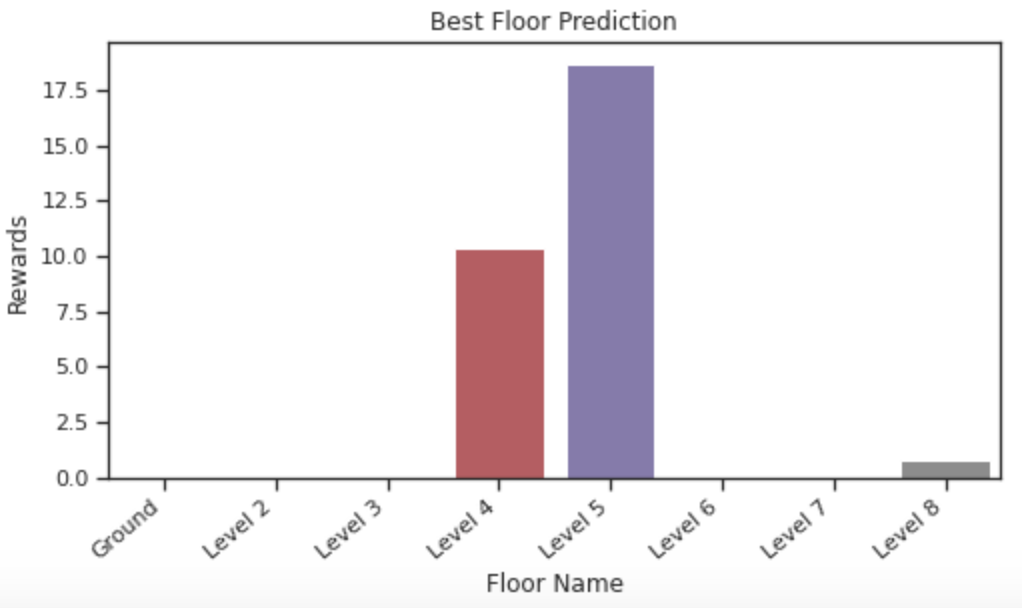
\includegraphics[width=10cm,keepaspectratio=true]{resources/images/floor_to/ian_no.png}
    \caption{Best rewarding floors of Ian Potter SouthBank Centre Building with no preference}
    \label{fig:ian_no}
    \end{figure}
    
    \item \textbf{Best nearby floors with high capacity:} From the Appendix Table \ref{appendix:ian_floor_to}, we find out that a student needs to walk at least \texttt{1 level} in the building to get rewarding floors with high capacity. It is also revealed that a relaxing parameter ($\delta$) of \texttt{2} can help students find highly rewarding floors. The result indicates that \texttt{Level 5} as the most rewarding floor with the cost of \texttt{2 floors} followed by \texttt{Level 4} with \texttt{3 floors} and \texttt{Level 3} with \texttt{4 floors} as shown in the Figure \ref{fig:ian_highcap}.
    
    \begin{figure}[H]
    \centering
    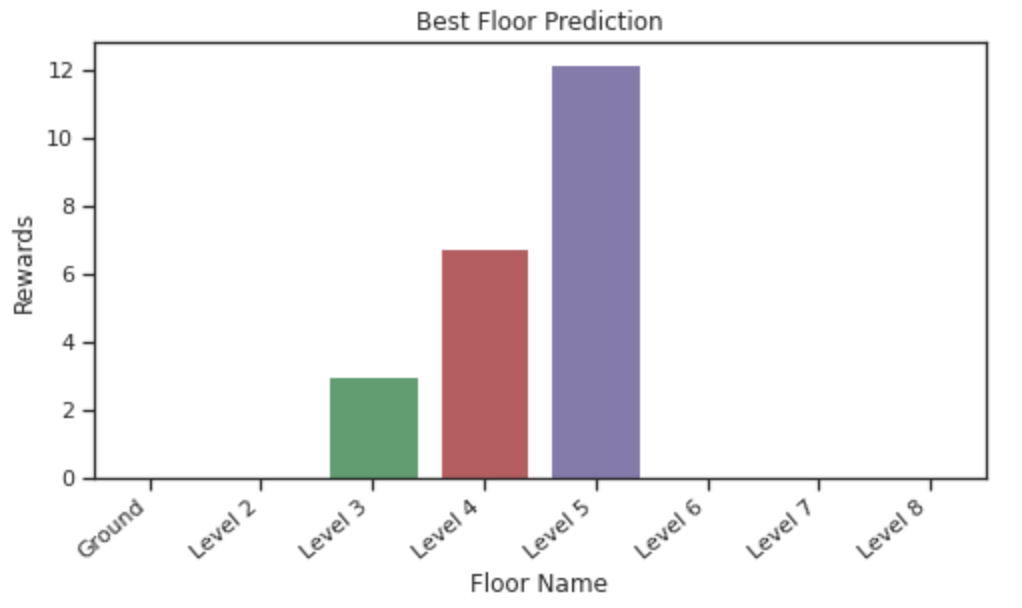
\includegraphics[width=10cm,keepaspectratio=true]{resources/images/floor_to/ian_highcap.png}
    \caption{Best rewarding floors of Ian Potter SouthBank Centre Building with high capacity}
    \label{fig:ian_highcap}
    \end{figure}
    
    \item \textbf{Best nearby floors with other factors:} We have also shown other factors such as finding toilets under COVID-19 Medium Lockdown or with easy availability in the Appendix Table \ref{appendix:ian_floor_to}. Using those constraints, we suggest that \texttt{Level 5} is the most rewarding floor with finding toilets with high capacity, or excellent condition. These are summarized in the below figures.
    
\begin{figure}[H]
\centering
\begin{subfigure}[b]{0.30\textwidth}
  \centering
  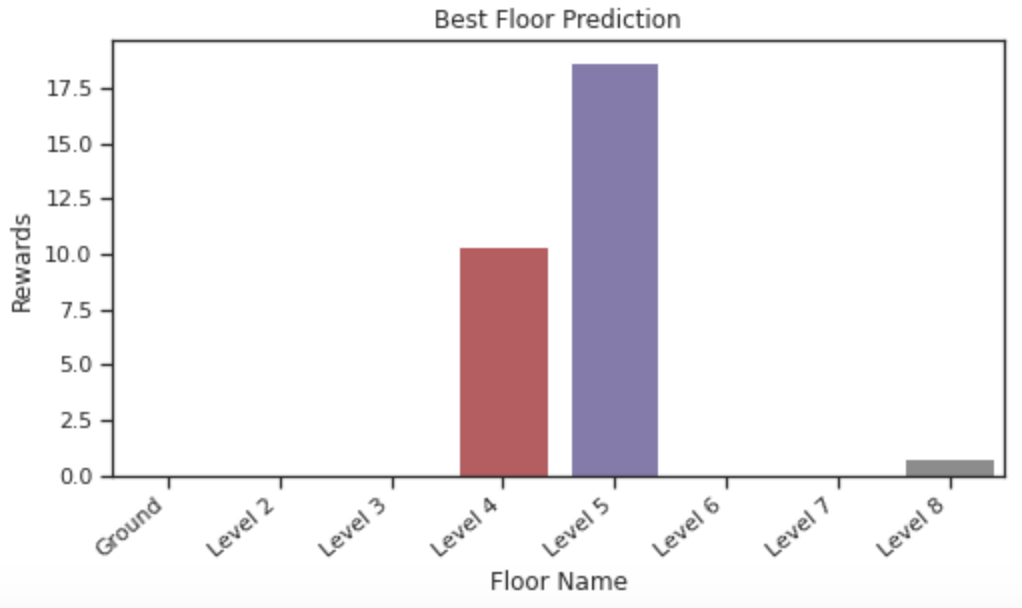
\includegraphics[width=5cm,keepaspectratio=true]{resources/images/floor_to/ian_covidmedium.png}
\end{subfigure}
\begin{subfigure}[b]{0.30\textwidth}
  \centering
  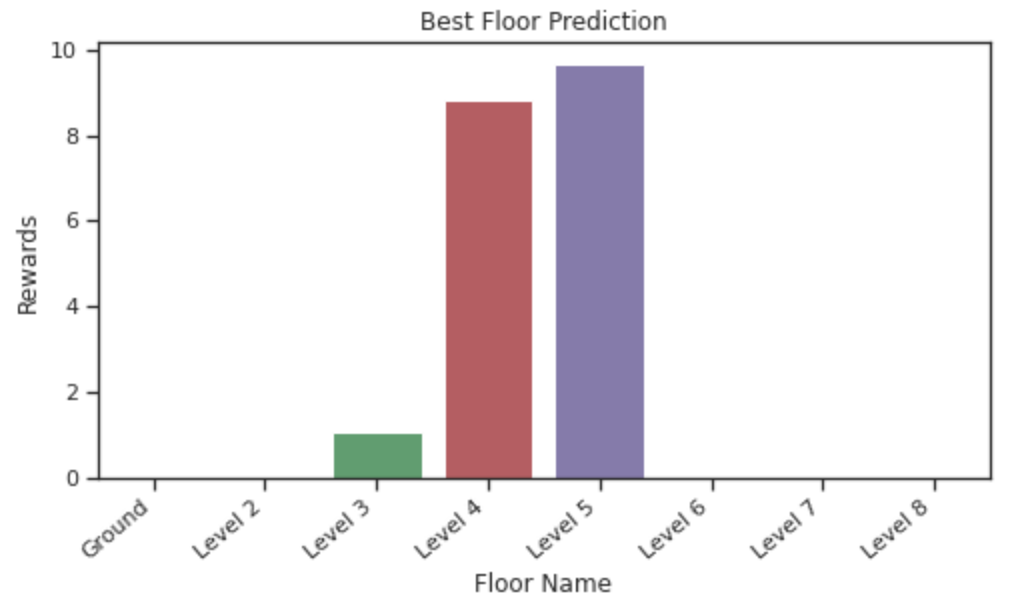
\includegraphics[width=5cm,keepaspectratio=true]{resources/images/floor_to/ian_easyava.png}
\end{subfigure}
\caption{Best rewarding floors of nearby floors of Old Microbiology under COVID-19 Medium Lockdown (left) and easy availability (right)}
\label{fig:ian-other-factors}
\end{figure}
    
\end{itemize}

